\documentclass[10pt,twocolumn,letterpaper]{article}

\usepackage{cvpr}
\usepackage{times}
\usepackage{epsfig}
\usepackage{graphicx}
\usepackage{amsmath}
\usepackage{amssymb}

% Include other packages here, before hyperref.

% If you comment hyperref and then uncomment it, you should delete
% egpaper.aux before re-running latex.  (Or just hit 'q' on the first latex
% run, let it finish, and you should be clear).
\usepackage[breaklinks=true,bookmarks=false]{hyperref}
\usepackage[english]{cleveref}

\cvprfinalcopy % *** Uncomment this line for the final submission

\def\cvprPaperID{MLCV Project 2017} % *** Enter the CVPR Paper ID here
\def\httilde{\mbox{\tt\raisebox{-.5ex}{\symbol{126}}}}

\graphicspath{{images/}}

\begin{document}

%%%%%%%%% TITLE
\title{Cutting Constraints on Conservation Tracking\\
  \large{Project Report MLCV Summer 2017}
}

\author{
Yuyan Li\\
{\tt\small yuyan.li@gmx.net}
\and
Kodai Matsuoka\\
{\tt\small kodaig06@gmail.com}
\and
Jui-Hung Yuan\\
{\tt\small j.yuan@stud.uni-heidelberg.de}
}

\maketitle
%\thispagestyle{empty}

\begin{abstract}
  Cell tracking exhibits multiple difficulties separating it from other tracking scenarios. The fact that cells can divide is one of them. Network flow methods in which divisions are integrated as constraints proved to be efficient at solving these problems. In our project we tried to improve the runtime performance of a network flow ILP by adding the division constraints successively, similar to the cutting planes algorithm. We demonstrate in experiments on two challenging datasets that only a fraction of all constraints are needed to solve the tracking. But because of the iterative nature of the method the gain in solving speed is outweight by the total time of the repeated solving.
\end{abstract}

\section{Introduction}

To understand the complex biological functions of living organisms, many experiments require monitoring of stem cells or bacteria over several generations under different conditions  \cite{elowitz2002stochastic, schroeder2011long}. However, those time-lapse experiments generate large amount of data, which human observers could hardly analyze without bias \cite{wu2010microscope}. Thus, automatated systems for cell tracking are necessary for those studies.

The analysis of the time-lapse microscopic results usually requires not only the tracking of position and locomotion of individual cells, but also the reconstruction of their full lineage \cite{amat2013towards}. In comparison to pedestrian tracking, the cell tracking task is more challenging due to the constant change of the cellular texture and morphology throughout the cell cycle, the high density of cells with uncertain movement as well as the division events which is not included in other multi-object tracking tasks.

To tackle the cell tracking task, a two-step pipeline \cite{yilmaz2006object} consisting of a segmentation/detection phase and an assignment/tracking phase is commonly used. In the first phase, the raw input images are segmented into foreground and background. Those segmentations and the raw data are then fed into classifiers that generate the corresponding detection and division hypotheses. Using the outputs of the classifiers as potentials, a graphical model is built for all possible assignments of  detection hypotheses between time frames in the second phase. Such tracking approaches are known as \textit{Tracking-by-assignment} methods \cite{bise2011reliable,padfield2011coupled}, which assume that the previous extracted set of detection hypotheses are over-complete and the constructed model thus describe all tracked targets. A globally consistent tracking solution is then reached via various optimization strategies.

The drawback of such method is that the errors in the first stage would propagate to, and warp, the tracking result. Such errors would occur where a cluster of objects is incorrectly represented by a single segment, termed as \textit{mergers} in this paper. To correct these over- and undersegmentation errors, the Conservation Tracking model \cite{schiegg2013conservation} which explicitly include the global consistency constraints was developed and was shown to outperform other tracking methods. From previous works, the Conservation Tracking model could be further reformulated into a constrained network flow problem which led to a tight LP relaxation and thus could be solved faster. Without the constraints for divisions and mergers, the LP relaxation of the model that accounts for flow conservation would yield integral solutions.

In our project we explored an method to exploit this last property and built an algorithm that disregards the division and merger constraints at first and only adds them to the model as needed.

\section{Constrained Network Flow Reformulation of Consveration Tracking}


\subsection{Conservation Tracking Model}

\begin{figure}[b]
  \begin{center}
    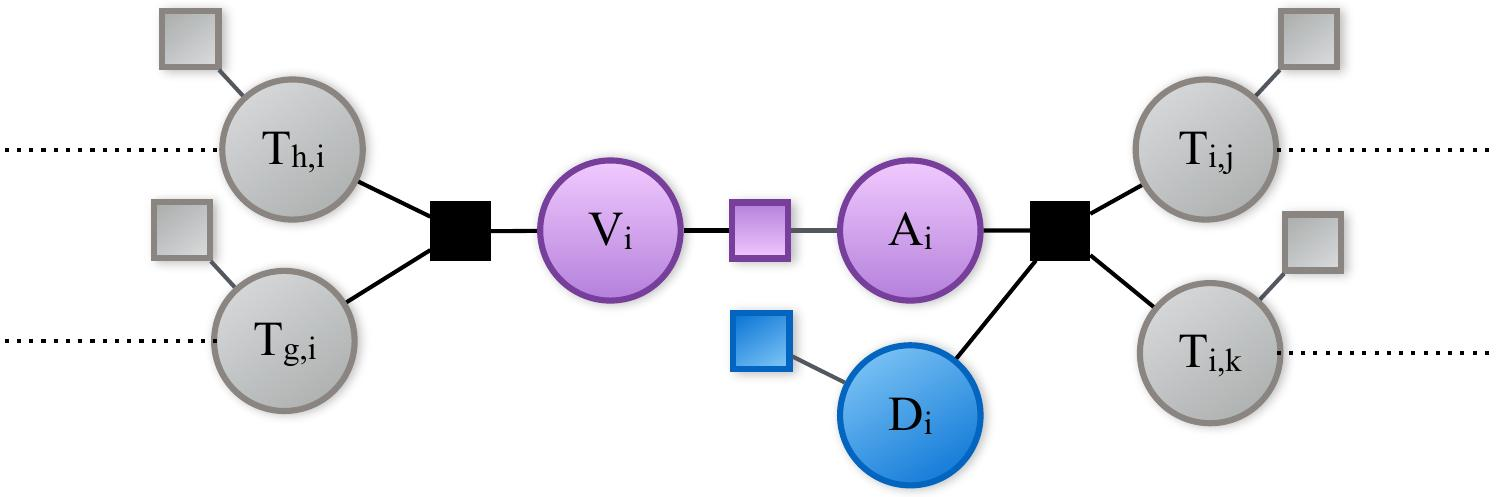
\includegraphics[width=0.8\linewidth]{model.jpeg}
    \caption{Factor graph for one detection with two incoming and two outgoing transition candidates. The circular nodes represent random variables, the non-black boxes describe factors that are dependent on the connected variables, and filled black boxes represent constraints. The purple detection node $i$ is seperated into a disappearance variable $V_i$ and an appearance variable $A_i$. The binary variable $D_i$ indicates whether object $i$ is about to divide. The transition variables $T \in \{0,...,m\}$ indicates the number of objects that are linked between two detection hypotheses.}
    \label{fig:ctmodel}
  \end{center}
\end{figure}

The Conservation Tracking model is presented in factor graphs as in Fig. \ref{fig:ctmodel}. The model contains three types of variables: \textit{Detection} variables $X_i \in \mathcal{X}$ (including the appearance $A_i \in \mathcal{A}$ and disappearance variables $V_i \in \mathcal{V}$) for each connected object from the segmented image, binary \textit{dividing} variables $D_i \in \mathcal{D}$ indicating whether an object is about to divide, and \textit{transition} variables $T_i \in \mathcal{T}$ that represent connections between the detections in two neighboring time frames. Noteworthy is that a division is allowed if and only if the corresponding detection contains one object. The probabilities of transition are modeled using the center of mass distance between detections, while the probabilities of appearance and disappearance are constant throughout time but linearly decrease to the edge of each image.

Let $\mathcal{Y}$ be the complete set of the configurations of all variables $\mathcal{V}\cup\mathcal{A}\cup\mathcal{T}\cup\mathcal{D}$, the approximate maximum a-posteriori (MAP) solution of the factor graph can be found by minimizing the energy
\scriptsize
\begin{equation}
\begin{split}
 y^* &= \operatorname*{arg\,max}_{y\in\mathcal{Y}} E(y) \\ 
     &= \operatorname*{arg\,max}_{y\in\mathcal{Y}} \sum\limits_{V\in\mathcal{V}}\sum\limits_{A\in\mathcal{A}} E_x(y_V, y_A) + \sum\limits_{T\in\mathcal{T}} E_T(y_T) + \sum\limits_{D\in\mathcal{D}} E_D(y_D)
\end{split}
\end{equation}
\normalsize
subject to constraints for flow conservation, division and mergers which will be explained in \ref{ILP formulation} in detail. This graphical model can be reformulated into a network flow and solved as an integer linear programming (ILP) problem.

\subsection{ILP for Network Flow}
\label{ILP formulation}

Linear Programming (LP) is a method to minimize (maximize) linear objective function, subject to linear inequality. Its formulation is as below.
\begin{align}
min_{x}  c^{T}x \\
s.t. Ax \leq b
\end{align}
The objective function \(c^{T}x\) linearly depends on the vector \(x \in R^{n}\) which represents n variables in question. Constraint \(Ax \leq b\) defines n hyperplanes that disallow x to lie in the back side. The area where x satisfies all the constraints is called "polytope". It is proved that the optimal solution lies on a vertex of the polytope. For this reason, LP is solved in polynomial time by searching along vertices on the polytope.
When x takes only integer values (i.e. \(x \in Z^{n}\) ), the problem is called Integer Linear Programs (ILP). ILP is NP hard in general and cannot be solved in polynomial time. 
A common approach to solve ILPs is to ignore the integrarity constraints and to solve this relaxed LP. Since this "relaxed" problem is LP, we can solve it in polynomial time. From the solution, we gain the information about original ILP problem.
If the solution of relaxed LP is integtal - and hence coinsides with the solution of original ILP - , the relaxation is said to be "tight" around the optimum.

A network flow is a directed graph with capacity on each edge. The flow can travel on directed graph under following rules. (1)The flow should not exceed the capacity. (2)The flow traveling to and from one node must be equal (Flow conservation). One can imagine as such networks water pipes, traffic network, electric circuits. There are several types of Network flow algorithms. For example, max-flow algorithm tries to maximize the flow from source to sink, and min-cost algorithm finds the route that minimize the cost. An important property here is that if all capacities are integers, optimal flow also takes an integer value. This situation corresponds to the constraint matrix(A) is totallly unimodular (TUM) in ILP, therefore LP relaxation is tight ~\cite{Bertsekas}.

\begin{figure}[t]
  \centering
  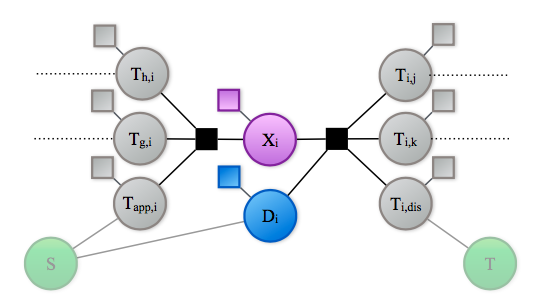
\includegraphics[width=0.8\linewidth]{model2.jpeg}
  \caption{In the constrained network flow graph, the detection node \(X_{i}\) is only a single node with unary factor, and appearances as well as disappearances are modeled as transitions \(T_{app,i}\) from an auxiliary source (green S ) or \(T_{i,dis}\) to an auxiliary sink (green T ) respectively.}
  \label{fig:ilpmodel}
\end{figure}

We deal with the flow network graph as shown in Fig. \ref{fig:ilpmodel} Notation is slightly changed from 2.1, $X_i \in \mathcal{X}$ is \textit{Detection} variables and the appearance $A_i \in \mathcal{A}$ and disappearance variables $V_i \in \mathcal{V}$ are modeled in \textit{transition} variables. Every random variables $V \in \mathcal{V}$ take state $k \in \mathcal{L}(V) \equiv {0, ...,m}$ indicating the number of contained target, where m is the upper about on the number of targets that can be merged into one detection. We introduce a unary potential $\theta_{V}(k)$ for every random variables $V \in \mathcal{V}$. This is the negative lof of probability that V takes value k. The probability is givein by local observation.
Our formulation is as follows.

\begin{scriptsize}
\begin{align}
  y^{*} &= \operatorname*{arg\,max}_{y\in\mathcal{Y}} E(y) \\ 
     &= \operatorname*{arg\,max}_{y\in\mathcal{Y}} \sum\limits_{X\in\mathcal{X}} E_X(y_X) + \sum\limits_{T\in\mathcal{T}} E_T(y_T) + \sum\limits_{D\in\mathcal{D}} E_D(y_D) \\
     &= \operatorname*{arg\,max}_{y\in\mathcal{Y}} \sum\limits_{X\in\mathcal{X}} \sum\limits_{k\in\mathcal{L(X)}} \theta_X(k) 1[y_X = k] \\
     & + \sum\limits_{T\in\mathcal{T}} \sum\limits_{k\in\mathcal{L(T)}} 1[y_T = k] \newline + \sum\limits_{D\in\mathcal{D}} \sum\limits_{k\in\mathcal{L(D)}} 1[y_D = k]
\end{align}
\text{subject to:} \\
\text{Flow conservarion:} \\
\begin{align}
\forall X\in\mathcal{X} \cup Sink : y_{X} = \sum\limits_{I\in\mathcal{I}(X)}y_{I}, \\
\forall X\in\mathcal{X} \cup Source : y_{X} + Y_{D(X)} = \sum\limits_{O\in\mathcal{O}(X)}y_{O}
\end{align}
\text{Division constraint:} \\
\begin{align}
\forall D\in\mathcal{D} : y_{D} - y_{X(D)} \leq 0
\end{align}
\text{Merger constraint:} \\
\begin{align}
\forall X\in\mathcal{X}, \forall I\in\mathcal{I}(X),I \neq App(X) : 1[y_{I}=0]+1[y_{App(X)}=0] \geq 1 \\
\forall X\in\mathcal{X}, \forall O\in\mathcal{O}(X),O \neq Dis(X) : 1[y_{O}=0]+1[y_{Dis(O)}=0] \geq 1
\end{align}
\end{scriptsize}

where $\mathcal{I}(X)$ is incoming to X, $\mathcal{O}(X)$ is outgoing. The meaning of each constraint is
flow conservation :the number of incoming and out going are the same.
division constraint :one cell can dicide into at most two cells.
merger constraint :mergers cannot partially disappear.

Because of these additional constraints, the TUM property collapses, so LP relaxation is not tight.
Therefore, we will first solve without division and meger constraints and then add only violated constraints.

\subsection{Cutting Constraints}

As stated before, we know that LP relaxation on the network flow without \textit{divisions} and \textit{mergers} will yield the optimal integral solution. Therefore we propose the following iterative alogrithm: In the first step the problem will be solved without division and merger constraints. Then, if there are flow conservation violation, the constraints are added for the relevant nodes. The last step is repeated until either a valid solution found or no new nodes with violations are found (leaving us with an invalid solution). This is done both with and without LP relaxation. Then as an variation, that makes use of the TUM property, we begin with LP relaxation and if the algorithm terminates without a valid solution it will continue with an ILP solver.


\subsection{Implementation}

We built our algorithm as an extension to the \textit{Multi Hypothesis Tracking} tool by Carsten \cite{haubold2017phd}. It is implemented in C++ and the inference was performed with Gurobi (although CPLEX can also be used). For the interface to Gurobi the OpenGM library \cite{opengm-library} for graphical models is used. The source code is available on \url{https://github.com/Ynzl/multiHypothesesTracking}.

\section{Experiments and Results}

We test our algorithm on two challenging datasets, a 3D+t drosophila scan (DRO) and 2D+t pancreatic rat stem cells (PSC) presented in Rapoport. There are two versions to both datasets, the full set including all mergers and a reduced version where mergers are omitted (DROr, PSCr). These datasets were given in the form of readily segmentated graphical models.

\subsection{Tracking Performance}

We track these datasets in five different ways. First we run the original tracking on the full model with all constraints added. We use this solution (referred to as \textit{Full}) as our baseline, \ie ground truth, to evaluate the tracking performance of the other runs. These are for the \textit{Cutting Constraint} algorithm (CC) and both experiments (Full and CC) run with LP relaxation. Lastly, the variation of \textit{Cutting Constraint} is used where it starts with LP relaxation and then switches to ILP (abbreviated with \textit{L2I} for LP to ILP).

\begin{table}
  \begin{center}
  \begin{tabular}{|l|c||c|c|c|}
    \hline
    Dataset & Nodes & \multicolumn{3}{|c|}{Constraints}\\
    \hline\hline
            &       & CC ILP & CC LP & L2I\\
    \hline
    DROr & 52k & 0 & 0 & 0\\
    PSCr & 118k & 86 & 133 & 2711\\
    DRO & 22k & 33 & 468 & 490\\
    PSC & 129k & 2605 & 15102 & 15867\\
    \hline
  \end{tabular}
  \end{center}
  \caption{Number of constraints added before the CC algorithm terminated. Note that the high number for the LP relaxation occur because non-integral numbers in the solution are also treated as flow violation. Thus division and merger constraints are added but do not improve the solution.}
  \label{tab:constraints}
\end{table}


Both the CC and L2I method produce valid tracking solutions. When using LP relaxation only the DROr dataset could be solved with a valid solution. \Cref{tab:constraints} shows that only a small amount nodes need to be submitted to the division and merger constraints to find a valid solution. Although this seems like a promising result, we will see in the runtime analysis that the time to find the constraints outweigh any speed improvement.

The quality of a solution is measured by comparing \textit{move}, \textit{merge} and \textit{division} events per pair of consecutive frames to the ground truth. The differences to the ground truth can be accounted by the allowed optimality gap of the Gurobi solver and the fact that the optimum must not be unique. The results in \cref{tab:fmeasure} indicate that the Cutting Constraint algorithm produces valid solutions that are very similar to the ground truth. Although the LP solutions seem to be close to the ILP ones they are not valid, with the exception of DROr.

\begin{table}
  \begin{center}
  \begin{tabular}{|l||c|c|c|c|}
    \hline
    Dataset & Full LP & CC ILP & CC LP & L2I\\
    \hline\hline
    DROr & 99.99 & 99.99 & 99.99 & 99.99\\
    PSCr & 99.91 & 99.93 & 99.92 & 99.92\\
    DRO & 99.22 & 99.99 & 99.28 & 99.99 \\
    PSC & 98.35 & 99.38 & 98.33 & 99.81\\
    \hline
  \end{tabular}
  \end{center}
  \caption{F-measure of the different tracking results with regard to the \textit{Full} ILP solution.}
  \label{tab:fmeasure}
\end{table}


\subsection{Runtime Analysis}

\begin{figure*}[t]
  \centering
  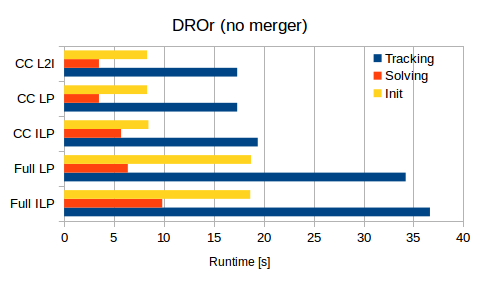
\includegraphics[width=.45\linewidth]{dror.png}
  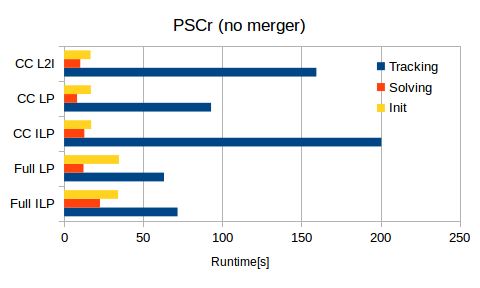
\includegraphics[width=.45\linewidth]{pscr.png}
  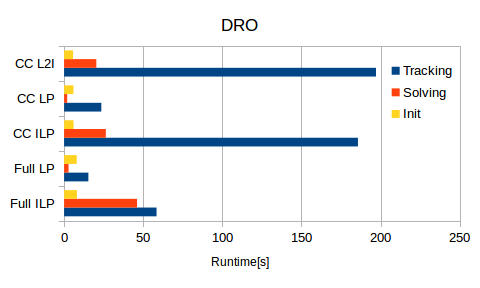
\includegraphics[width=.45\linewidth]{dro.png}
  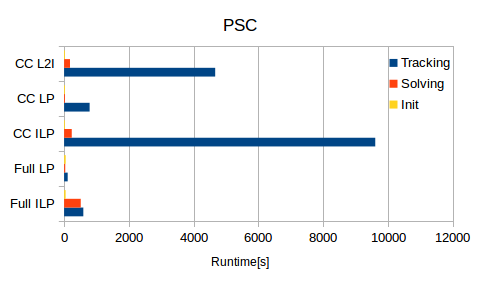
\includegraphics[width=.45\linewidth]{psc.png}
  \caption{Runtime of the different tracking methods. In blue the total tracking time, in red the solving time which is the average over all iterations for the CC runs, in yellow the time to initialize the graphical model in OpenGM.}
  \label{fig:runtime}
\end{figure*}

    The runtime of the different methods are shown in \cref{fig:runtime}. All timings were performed on a machine with an Intel Core i7-6700HQ with 8 cores at 2.6GHz and 8GB RAM. Each experiment was run three times and the median is presented. In most cases the deviation between the runs was very small ($\sigma \leq 5\%$). However the size of the PSC model forced the machine to its limits and lead to big variations in the runtime. Furthermore because the black-box nature of both the Gurobi solver and the operating system it ran on, the runtime could be influenced by diverse mechanism unknown to us. Ideally the experiments are done on a machine with a lot more RAM. For the CC method the solving time is taken as the average over all iterations. In the L2I case this is not meaningful because of the mixing of ILP and LP solving.

    The experiments show that cutting constraints improve both model initialization time and the solving time significantly. But because of the amount of iterations (see \cref{tab:iter}) and the time to verify the intermediate solutions, the total tracking time is slower. An exception is the DROr dataset without mergers which can be solved without any division constraints. For all other datasets the needed constraints were only found after a significant amount of iterations.

\begin{table}
  \begin{center}
  \begin{tabular}{|l||c|c|c|c|}
    \hline
    Dataset & CC ILP & CC LP & L2I\\
    \hline\hline
    DROr & 1 & 1 & 1 \\
    PSCr & 8 & 4 & 7 \\
    DRO & 6 & 3 & 8 \\
    PSC & 38 & 14 & 23 \\
    \hline
  \end{tabular}
  \end{center}
  \caption{Number of iterations for the different CC runs.}
  \label{tab:iter}
\end{table}

The iteration numbers of the L2I runs show that CC LP does not find all needed division and merger constraints. While L2I show a small improvement in runtime over CC ILP it still is much slower than the Full run.

\section{Conclusion}

Based on the constrained network flow formulation of conservation tracking we explored a method to relax on division and merger constraints for cell tracking. We have shown that only a small fraction of all constraints are needed to find a valid tracking solution. Additionally, once the needed constraints are found the tracking takes less time. But because the needed constraints are only found after a lot of iterations, our cutting constraint algorithm proved to be slower and thus inefficient. Further exploratory development could be done by implementing the algorithm directly into the ILP solver avoiding the overhead made by the OpenGM framework.


{\small
\bibliographystyle{ieee}
\bibliography{bib}
}

\end{document}
